\begin{sie}
 \chapter{Toward a quantitative theory of Hofmeister effects: from quantum effects to thermodynamics}
 \hyperlink{toc}{Return to TOC}
  \section{\label{ch3:sec0:level1}Preface}
  This chapter draws text and data from a published article,
  
  \vspace{12pt}
  \noindent \emph{Travis P.~Pollard, Thomas L.~Beck, Toward a quantitative theory of Hofmeister phenomena: From quantum effects to 
  thermodynamics, Current Opinion in Colloid $\&$ Interface Science, Volume 23, June 2016, Pages 110-118.}
  \vspace{12pt}
  
  \noindent Additional data is supplied here that will be published in a forthcoming article. 
  
  These articles concern the local solvation structure around the alkali/halide ions which is critical in developing a quantitative 
  theory of the specific ion effects discussed throughout Chapter \ref{ch1:sec1:level1}. This is because the solvation structure is
  shaped not only by electrostatic forces but also dispersion and induction contributions, which requires electronic resolution. Recent 
  simulation work has also observed that charge transfer between anions to surrounding waters decreases overall solvation asymmetry. 
  I sought to explore the relationship between solvation structure and the presence of these non-electrostatic forces. To do this, I 
  carried out a series of electronic structure calculations to optimize myriad X$^{\pm}$(H$_{2}$O)$_{n}$ clusters, where X is one of 
  Li$^{+}$, Na$^{+}$, K$^{+}$, F$^{-}$, Cl$^{-}$, or Br$^{-}$, and \emph{n} = 1, \dots, 6. Following this, I used the symmetry adapted 
  perturbation theory (discussed in Chapter \ref{ch2:sec2:level1}) to extract interaction energies and components. Energies are complemented
  with the use of quantum theory of atoms in molecules to estimate the ion charge from gas phase to several states with a (nearly) 
  completed first solvation shell. From this I learned that dispersion and induction forces make up approximately $\frac{1}{3}$ of
  the attractive contributions to the interaction energy for anion/water clusters -- though, these effects tended to (nearly) saturate
  within the first shell regardless of ion charge. I also discovered that the symmetry adapted perturbation theory is not suitable to 
  estimating the stabilization energy of ion/water complexes due to partial charge transfer. However, I proposed that it may be better 
  suited to providing an upper bound on the polarization energy. Combined with the polarized orthogonally localized molecular orbital
  method, the polarization energy can be bounded from below too (this likewise produces upper and lower bounds to the charge transfer 
  energy). However, assuming the relative values for a given ion and cluster size were qualitatively correct, I found that for 
  F$^{-}$(H$_{2}$O)$_{6}$, the charge transfer interaction energy favored clusters where the ion was internally solvated (as opposed
  to surface solvated). This is consistent with the findings of others which suggest that the inclusion of partial charge transfer 
  in simulation promotes the reduction of solvent distribution anisotropy around the ion.
  
  This section addresses three of the questions I posed in Chapter \ref{ch1:sec1:level4},

  \begin{itemize}
      \item What sort of interactions? 
      \item How strong are they relative to one another?
      \item Do we need electronic structure theory to solve everything?
      \item Will a simpler model work far away from the ion?
  \end{itemize}
  
  \section{\label{ch3:sec1:level1}Computational methods}
  This chapter covers the findings outlined in two separate studies. In this case, the studies share a significant degree of overlap so a 
  combined methods section is covered below.
  
   \subsection{\label{ch3:sec1:level2}Optimization and atomic partial charges}
    Small ion/water clusters were optimized to the SCS-MP2/CVTZ level of theory\cite{grimme2003scsmp2} (details of the basis sets used are 
    explained later) using the Orca 3.0.3 quantum chemistry package\cite{neese2012orca,valeev2014libint}. A number of favorable initial 
    geometries were extracted from the literature for each cluster size to explore the variation in charge transfer that accompanies partial 
    solvation\cite{kim1999bigf,kim2000smallall,kim2002bigall}. Molden-type inputs of the MP2 natural orbitals were converted 
    to standard wave function files (WFN) using the molden2aim script available here, (\url{http://people.smu.edu/wzou/program/}). The electron 
    density was partitioned by computing the so-called zero-flux surface about the ion within the framework of the quantum theory of atoms 
    in molecules (AIM) pioneered by Bader\cite{bader1990book}. Calculations were carried out for each of the complexes and also the isolated 
    fragments with the difference in the net charge values taken as an estimate of the charge exchanged upon complexation. AIM calculations 
    were performed using the AIMAll package\cite{bader1982proaim,keith2012aimall}. All data necessary for visualization of electron 
    density surfaces or contours were generated using Multiwfn\cite{lu2012multiwfn} and viewed using VMD\cite{humphrey1996vmd} (surface) or the 
    native plotting utility in Multiwfn (contours).

   \subsection{\label{ch3:sec1:level3}Energy decomposition using symmetry adapted perturbation theory}
    Interaction energies were computed at the density fit SCS-MP2 level of theory with counterpoise corrections\cite{boys1970bsse} and the 
    SAPT2+3(CCD)\cite{jeziorski1994sapt,hohenstein2010df,hohenstein2012sapt} level of theory using the open source Psi4\cite{sherrill2012psi4} 
    software. We report the error in the exchange-induction coupled terms at 2\sur{nd}- and 3\sur{rd}-orders of SAPT but otherwise do not scale the
    affected terms as discussed elsewhere in the literature\cite{hohenstein2011scale,herbert2012break}. Errors in the SAPT energies relative
    to SCS-MP2 are in the neighborhood of 6-8\% for the largest cluster sizes with SAPT almost always overshooting the counterpoise-corrected 
    estimate.
    
   \subsection{\label{sec3:sec1:level4}The charge transfer energy}
    The Hellmann-Feynman theorem states that once an electron distribution has been solved, all forces within the system can be calculated
    purely through classical electrostatics and the Coulomb operator. Partitioning of these energies has a physical basis but is purely
    `modeling' in many cases\cite{politzer2015mathematical}. However, this modeling is imported into classical force fields which tends to 
    make them more accurate and so it is instructive to partition energies into separable components in an attempt to translate them to simpler
    force field based simulation. As an interesting aside, non-variational methods (e.g., MP2) do not satisfy the Hellmann-Feynman theorem\cite{jensen2013introduction}.
    Nevertheless, charge transfer contributions to the interaction energy between ion/water clusters were modeled using a pair of partitioning schemes
    within the symmetry adapted perturbation theory (SAPT)\cite{jeziorski1994sapt}. We'll refer to these methods as SM09 and reg-SAPT. The
    SM09 method was outlined by Stone et al. and entails taking the difference in the induction energy to arbitrary order between a dimer-
    centered and monomer-centered basis set calculation\cite{stone2009ct}. In this case, charge transfer is modeled only as a basis set 
    superposition error artifact and so vanishes in the limit of a complete basis. Recent work by Lande et al. has shown this method to be 
    most `reliable' for moderate-sized basis sets, e.g., aug-cc-pVTZ\cite{lande2015cdftct}. To overcome the shortcomings of the SM09 method,
    Misquitta replaced the monomer-centered basis calculation with one in which the nuclear potential of each fragment is screened from the
    opposite\cite{misquitta2013regsapt}. Inclusion of the screening potential prevents charge transfer but allows for polarization. The sole 
    adjustable parameter in the method is the length scale of the screening potential which is modeled as a Gaussian \emph{s}-orbital with
    width, $\eta$. Misquitta found that $\eta =$ 3.0 au (units are L\sur{-2}) was sufficient for most applications involving the first and 
    second row elements\cite{misquitta2013regsapt}. The parameter is tuned by minimizing the difference in the total induction energy,
    E\sursous{(2)}{ind,tot}, between the dimer- and monomer-centered basis over a range of intermolecular separations, including some points
    below the equilibrium bond length. Tuning was only done for ion/water dimers. Anions presented a bit of a challenge in that the differences
    varied little with changes in the width of the screening orbital. We selected the value in the range of $\eta =$ 1.0 au to 3.0 au which
    also minimized the change in E\sursous{(2)}{ind,tot} computed with the dimer-centered basis set alone. Once a range parameter is determined,
    the charge transfer energy is simply equal to the difference in induction energies computed with and then without the conditioning, both
    using a dimer-centered (or extended monomer-centered) basis representation. These energies exhibit significantly less variance with 
    increasing basis set size. SM09 calculations were performed up to the SAPT2 level using the cc-pVTZ (+ diffuse, where appropriate and 
    def2-TZVPP for K\sur{+})\cite{dunning1989h,dunning1992of,dunning1993cl,dunning1999br,hattig2002ri,rappoport2010def2,rappoport2015kri}
    with the Psi4 package\cite{sherrill2012psi4,hohenstein2010df,hohenstein2012sapt}. Regularized SAPT was handled with the regSAPT
    script included in the SAPT2008 package\cite{jeziorski2012sapt}. The rather dated ATMOL1024 SCF interface\cite{saundersatmol} to the SAPT2008 
    package required an additional change in basis set due to small contraction and total orbital limits. All clusters were successfully modeled with 
    (aug-)cc-pVDZ (Feller's CVDZ) and the (aug-)pc-1 polarization consistent basis 
    set\cite{jensen2001principles,jensen2002diffusefxns,jensen2004cl,jensen2007lina,jensen2012kbr}. However we 
    addressed optimization of the regularization length scale with the def2-QZVPP (+ diffuse, where appropriate) basis\cite{rappoport2010def2}
    and these results are listed in Table \ref{tab:ion_params}. All basis sets were retrieved from the EMSL Basis Set Exchange\cite{emsl1996,emsl2007}.
    
\begin{table}
 \begin{center}
  \begin{tabular}{lc}
   \hline
   \hline
    A & $\eta$ \tabularnewline
   \hline
    H         & 3.0  \tabularnewline
    Li\sur{+} & 3.0  \tabularnewline
    O         & 3.0  \tabularnewline
    F\sur{-}  & 2.5  \tabularnewline
    Na\sur{+} & 3.0  \tabularnewline
    Cl\sur{-} & 1.5  \tabularnewline
    K\sur{+}  & 1.5  \tabularnewline  
    Br\sur{-} & 1.5  \tabularnewline 
   \hline 
   \hline
  \end{tabular}
 \end{center}
 \caption[Optimal range parameters for regularizing potential]{\label{tab:ion_params} Optimal $\eta$ parameters for each element in atomic units ($\eta$ 
 has units of L\sur{-2}). These results support the conclusion of Misquitta that an $\eta$ value near 3.0 au produces adequate screening for the first and 
 second row elements.}
 \end{table}

   \subsection{\label{ch3:sec1:level5}Basis sets}
    Geometry optimization and subsequent generation of WFN files for use with the AIMAll package was carried out with a triple-$\zeta$ quality 
    basis with core-valence functions included for second row and beyond elements 
    (aug-cc-pwCVTZ)\cite{dunning1989h,peterson2002ofcl,peterson2007br,peterson2011lina}. Diffuse functions were removed from the 
    cation basis sets to be consistent with K\sur{+} which had to be modeled with Feller's CVTZ\cite{feller1995k} due to a lack of parameterization 
    in the Dunning sets. The emphasis on density fitting algorithms in Psi4 ultimately required us to pursue the valence-only flavors of the preceding
    basis sets (we substituted the def2-TZVPP basis in for K\sur{+} calculations\cite{rappoport2010def2,rappoport2015kri}). For density fit procedures 
    a Cholesky decomposed basis was constructed with a tolerance 1e-4.
    
  \section{\label{ch3:sec2:level1}Results $\&$ Discussion}
  \subsection{\label{ch3:sec2:level1:chasm1}Interaction energies, atoms in molecules, and partial charges}
  I begin with a survey of the SAPT2+3 (CCD) interaction energies for clusters with up to 6 attached waters, see  Tables \ref{tab:sapt1}--\ref{tab:sapt4}. 
  Even a cursory look over these data confirms the presence of a great deal of ion specificity across all of the components of the interaction energies 
  -- especially in the induction and dispersion contributions for F\sur{-} clusters relative to both Cl\sur{-} and Br\sur{-}.

\begin{table}
 \begin{center}
 \begin{tabular}{lrrrrccrr}
   Cluster & Elst & Ind & Disp & Exch & Exch Err & E\sur{PT} & E\sur{CP} \tabularnewline
  \hline
  \tabularnewline
   \multicolumn{8}{c}{\textbf{X\sur{\pm}(H\sous{2}O)}}  \tabularnewline
  \tabularnewline
Li\sur{+} C\sous{2v} &-32.90 &-13.52 &-0.68 &12.55 &1.00 &-34.56 &-33.46 \tabularnewline
Na\sur{+} C\sous{2v} &-24.95 & -6.39 &-0.43 & 8.43 &1.00 &-23.33 &-22.53 \tabularnewline
K\sur{+}  C\sous{2v} &-19.73 & -4.78 &-1.73 & 8.73 &1.01 &-17.51 &-16.63 \tabularnewline
F\sur{-}  C\sous{1}  &-44.50 &-29.26 &-7.80 &49.33 &1.03 &-32.23 &-29.35 \tabularnewline
Cl\sur{-} C\sous{1}  &-19.01 & -7.57 &-4.42 &15.41 &1.01 &-15.58 &-14.24 \tabularnewline
Br\sur{-} C\sous{1}  &-16.35 & -6.03 &-4.15 &13.13 &1.01 &-13.39 &-12.18 \tabularnewline
  \tabularnewline
   \multicolumn{8}{c}{\textbf{X\sur{\pm}(H\sous{2}O)\sous{2}}}  \tabularnewline
  \tabularnewline
Li\sur{+} D\sous{2d} &-60.95 &-24.85 & -1.36 &20.85 &1.01 &-66.31 &-63.79 \tabularnewline
Na\sur{+} D\sous{2d} &-47.26 &-12.09 & -0.79 &14.76 &1.00 &-45.38 &-43.76 \tabularnewline
K\sur{+}  D\sous{2d} &-36.63 & -8.05 & -3.10 &14.04 &1.00 &-33.74 &-32.13 \tabularnewline
F\sur{-}  C\sous{2}  &-71.95 &-37.84 &-11.76 &69.29 &1.01 &-52.25 &-48.95 \tabularnewline
Cl\sur{-} C\sous{1}  &-35.03 &-13.09 & -8.02 &26.53 &1.02 &-29.62 &-27.05 \tabularnewline
Br\sur{-} C\sous{1}  &-30.37 &-10.64 & -7.58 &22.82 &1.02 &-25.78 &-23.42 \tabularnewline
  \tabularnewline
   \multicolumn{8}{c}{\textbf{X\sur{\pm}(H\sous{2}O)\sous{3}}}  \tabularnewline
  \tabularnewline
Li\sur{+} D\sous{3}      &-82.63 &-33.99 & -1.82 &24.70 &1.01 &-93.74 &-89.70 \tabularnewline
Li\sur{+} 2+1(C\sous{2}) &-71.65 &-26.84 & -1.42 &21.88 &1.01 &-78.03 &-75.15 \tabularnewline
Na\sur{+} D\sous{3}      &-66.13 &-17.10 & -1.14 &18.88 &1.00 &-65.49 &-62.92 \tabularnewline
Na\sur{+} 2+1(C\sous{2}) &-56.86 &-13.26 & -0.92 &16.08 &1.00 &-54.95 &-52.99 \tabularnewline
K\sur{+}  D\sous{3}      &-52.40 &-11.43 & -4.47 &18.98 &1.00 &-49.32 &-46.89 \tabularnewline
K\sur{+}  2+1(C\sous{2}) &-46.20 &-10.08 & -3.57 &17.07 &1.01 &-42.78 &-40.76 \tabularnewline
F\sur{-}  C\sous{3}      &-89.25 &-40.46 &-14.48 &75.84 &1.00 &-68.46 &-64.43 \tabularnewline
F\sur{-}  2+1(C\sous{s}) &-86.00 &-42.36 &-12.72 &75.89 &1.01 &-65.19 &-61.48 \tabularnewline
Cl\sur{-} C\sous{3}      &-48.54 &-16.14 &-10.92 &33.74 &1.01 &-41.86 &-38.20 \tabularnewline
Cl\sur{-} 2+1(C\sous{s}) &-45.72 &-16.48 & -9.34 &32.49 &1.01 &-39.05 &-36.16 \tabularnewline
Br\sur{-} C\sous{3}      &-42.52 &-13.36 &-10.47 &29.58 &1.02 &-36.77 &-33.33 \tabularnewline
Br\sur{-} 2+1(C\sous{s}) &-40.03 &-13.63 & -8.91 &28.20 &1.01 &-34.37 &-31.69 \tabularnewline
  \hline
 \end{tabular}
 \end{center}
 \caption[Interaction energies for ion/water clusters with \emph{n} = 1, 2, and 3]{\label{tab:sapt1} SAPT2+3(CCD) energy decomposition: 
 electrostatics (Elst), induction (Ind), dispersion (Disp), exchange (Exch), 
 and total interaction energy (E\sur{PT}) in the dimer-centered aug-cc-pVTZ basis set. All energies expressed in kcal/mol. Exch Err is a 
 value quantifying the degree of error in the single-exchange approximation which affects the accuracy of exchange-coupled higher order 
 induction terms. A value greater than unity indicates an overestimation of the induction energy and vice versa. This figure represents
 a large source of error in the difference between E\sur{PT} and the conventional counterpoise-corrected interaction energy, E\sur{CP}.}
\end{table}

\begin{table}
 \begin{center}
 \begin{tabular}{lrrrrccrr}
   Cluster & Elst & Ind & Disp & Exch & Exch Err & E\sur{PT} & E\sur{CP} \tabularnewline
  \hline
  \tabularnewline
   \multicolumn{8}{c}{\textbf{X\sur{\pm}(H\sous{2}O)\sous{4}}}  \tabularnewline
  \tabularnewline
Li\sur{+} S\sous{4}                  & -98.29 &-40.57 & -2.16 &24.38 &1.01 &-116.64 &-111.20 \tabularnewline
Li\sur{+} 3+1(C\sous{2})             & -93.67 &-34.78 & -1.53 &25.39 &1.01 &-104.59 &-101.11 \tabularnewline
Na\sur{+} S\sous{4}                  & -82.16 &-21.50 & -1.60 &21.40 &1.00 & -83.87 &-80.29 \tabularnewline
Na\sur{+} 3+1(C\sous{2})             & -75.69 &-18.12 & -1.23 &19.93 &1.00 & -75.11 &-72.30 \tabularnewline
K\sur{+}  S\sous{4}                  & -66.01 &-14.33 & -5.65 &22.31 &1.00 & -63.70 &-60.47 \tabularnewline
K\sur{+}  3+1(C\sous{2})             & -60.66 &-12.37 & -4.71 &20.16 &1.00 & -57.58 &-54.92 \tabularnewline
F\sur{-}  C\sous{1}                  &-107.86 &-42.49 &-16.68 &83.45 &0.99 & -83.59 &-79.51 \tabularnewline
F\sur{-}  C\sursous{\prime\prime}{1} &-108.26 &-43.64 &-16.84 &85.30 &0.99 & -83.43 &-79.41 \tabularnewline
F\sur{-}  C\sous{4}                  &-102.93 &-42.06 &-16.34 &78.96 &1.00 & -82.37 &-78.06 \tabularnewline
F\sur{-}  3+1(C\sous{s})             &-105.96 &-45.02 &-15.28 &85.82 &1.00 & -80.45 &-76.79 \tabularnewline
Cl\sur{-} C\sursous{\prime}{1}       & -61.65 &-19.84 &-13.70 &41.32 &1.01 & -53.87 &-49.27 \tabularnewline
Cl\sur{-} C\sursous{\prime\prime}{1} & -60.60 &-19.18 &-13.39 &40.60 &1.01 & -52.58 &-48.23 \tabularnewline
Cl\sur{-} C\sous{4}                  & -58.94 &-18.16 &-13.03 &38.07 &1.01 & -52.06 &-47.69 \tabularnewline
Br\sur{-} C\sursous{\prime}{1}       & -54.42 &-16.90 &-13.27 &36.81 &1.02 & -47.79 &-43.38 \tabularnewline
Br\sur{-} C\sursous{\prime\prime}{1} & -53.35 &-16.23 &-12.93 &36.06 &1.01 & -46.45 &-42.30 \tabularnewline
Br\sur{-} C\sous{4}                  & -51.90 &-15.12 &-12.60 &33.78 &1.01 & -45.84 &-41.67 \tabularnewline
  \hline
 \end{tabular}
 \end{center}
 \caption[Interaction energies for ion/water clusters with \emph{n} = 4]{\label{tab:sapt2} SAPT2+3(CCD) energy decomposition: electrostatics 
 (Elst), induction (Ind), dispersion (Disp), exchange (Exch), 
 and total interaction energy (E\sur{PT}) in the dimer-centered aug-cc-pVTZ basis set. All energies expressed in kcal/mol. Exch Err is a 
 value quantifying the degree of error in the single-exchange approximation which affects the accuracy of exchange-coupled higher order 
 induction terms. A value greater than unity indicates an overestimation of the induction energy and vice versa. This figure represents
 a large source of error in the difference between E\sur{PT} and the conventional counterpoise-corrected interaction energy, E\sur{CP}.}
\end{table}

\begin{table}
 \begin{center}
 \begin{tabular}{lrrrrccrr}
   Cluster & Elst & Ind & Disp & Exch & Exch Err & E\sur{PT} & E\sur{CP} \tabularnewline
  \hline
  \tabularnewline
   \multicolumn{8}{c}{\textbf{X\sur{\pm}(H\sous{2}O)\sous{5}}}  \tabularnewline
  \tabularnewline
Li\sur{+} C\sous{2}        &-106.66 &-41.11 & -1.60 &19.44 &1.01 &-129.93 &-124.73 \tabularnewline
Li\sur{+} 4+1(C\sous{2})   &-108.62 &-40.76 & -1.79 &24.97 &1.01 &-126.20 &-121.46 \tabularnewline
Na\sur{+} 4+1(C\sous{2})   & -90.97 &-22.37 & -1.64 &22.05 &1.00 & -92.92 &-89.12 \tabularnewline
Na\sur{+} C\sous{2}        & -84.15 &-24.06 & -1.91 &19.92 &1.00 & -90.20 &-85.82 \tabularnewline
K\sur{+}  4+1(C\sous{2})   & -73.70 &-14.96 & -5.79 &22.77 &1.00 & -71.68 &-68.29 \tabularnewline
K\sur{+}  C\sous{2}        & -58.86 &-15.09 & -5.93 &18.47 &1.00 & -59.40 &-55.81 \tabularnewline
K\sur{+}  4+1(C\sous{1})   & -53.79 &-14.49 & -5.40 &18.92 &1.00 & -54.76 &-51.39 \tabularnewline
F\sur{-}  R3L2             &-119.58 &-43.83 &-18.43 &85.14 &0.99 & -96.70 &-92.03 \tabularnewline
F\sur{-}  R4L              &-118.12 &-43.22 &-18.07 &83.61 &0.99 & -95.80 &-91.37 \tabularnewline
F\sur{-}  L3DL             &-114.53 &-46.02 &-17.39 &86.66 &1.00 & -91.29 &-86.80 \tabularnewline
F\sur{-}  R4A              &-112.76 &-44.37 &-17.10 &83.54 &1.00 & -90.69 &-86.17 \tabularnewline
F\sur{-}  R43f             &-111.75 &-44.42 &-16.99 &83.17 &1.00 & -89.98 &-85.50 \tabularnewline
F\sur{-}  R4L\sur{\prime}  &-112.94 &-44.56 &-17.05 &86.16 &0.99 & -88.39 &-84.17 \tabularnewline
F\sur{-}  R3AA             &-109.36 &-47.27 &-15.78 &86.30 &1.00 & -86.12 &-81.89 \tabularnewline
Cl\sur{-} R4A1             & -67.14 &-22.32 &-14.67 &44.79 &1.01 & -59.34 &-54.53 \tabularnewline
Cl\sur{-} R4A              & -66.57 &-21.19 &-14.36 &43.35 &1.01 & -58.77 &-54.07 \tabularnewline
Cl\sur{-} R43f             & -65.47 &-20.92 &-14.13 &42.65 &1.01 & -57.88 &-53.30 \tabularnewline
Cl\sur{-} R3AA\sur{\prime} & -63.09 &-22.16 &-12.98 &43.02 &1.01 & -55.21 &-51.15 \tabularnewline
Cl\sur{-} R5               & -61.92 &-20.16 &-13.65 &40.66 &1.01 & -55.07 &-50.59 \tabularnewline
Cl\sur{-} R3AA             & -62.01 &-22.20 &-12.86 &42.35 &1.01 & -54.71 &-50.59 \tabularnewline
Cl\sur{-} R4f3             & -62.03 &-22.21 &-12.87 &42.40 &1.01 & -54.71 &-50.58 \tabularnewline
Br\sur{-} R4A1             & -59.22 &-19.09 &-14.29 &40.00 &1.01 & -52.61 &-47.96 \tabularnewline
Br\sur{-} R4A              & -59.07 &-18.20 &-14.06 &39.07 &1.01 & -52.27 &-47.72 \tabularnewline
Br\sur{-} R43f             & -57.89 &-17.84 &-13.78 &38.22 &1.01 & -51.29 &-46.89 \tabularnewline
Br\sur{-} R3AA\sur{\prime} & -55.46 &-18.89 &-12.57 &38.02 &1.01 & -48.90 &-45.03 \tabularnewline
Br\sur{-} R5               & -54.46 &-16.94 &-13.25 &36.16 &1.01 & -48.49 &-44.21 \tabularnewline
Br\sur{-} R4f3             & -54.40 &-18.89 &-12.41 &37.29 &1.02 & -48.41 &-44.89 \tabularnewline
  \hline
 \end{tabular}
 \end{center}
 \caption[Interaction energies for ion/water clusters with \emph{n} = 5]{\label{tab:sapt3} SAPT2+3(CCD) energy decomposition: electrostatics
 (Elst), induction (Ind), dispersion (Disp), exchange (Exch), 
 and total interaction energy (E\sur{PT}) in the dimer-centered aug-cc-pVTZ basis set. All energies expressed in kcal/mol. Exch Err is a 
 value quantifying the degree of error in the single-exchange approximation which affects the accuracy of exchange-coupled higher order 
 induction terms. A value greater than unity indicates an overestimation of the induction energy and vice versa. This figure represents
 a large source of error in the difference between E\sur{PT} and the conventional counterpoise-corrected interaction energy, E\sur{CP}.}
\end{table}

\begin{table}
 \begin{center}
 \begin{tabular}{lrrrrccrr}
   Cluster & Elst & Ind & Disp & Exch & Exch Err & E\sur{PT} & E\sur{CP} \tabularnewline
  \hline
  \tabularnewline
   \multicolumn{8}{c}{\textbf{X\sur{\pm}(H\sous{2}O)\sous{6}}}  \tabularnewline
  \tabularnewline
Li\sur{+} D\sous{2d}      &-118.06 &-42.73 & -2.22 &24.80 &1.01 &-138.22 &-132.30 \tabularnewline
Li\sur{+} 4+2(C\sous{s})  &-116.73 &-42.62 & -2.22 &25.07 &1.01 &-136.49 &-130.58 \tabularnewline
Li\sur{+} C\sous{2}       &-100.80 &-42.33 & -2.17 &24.59 &1.01 &-120.71 &-114.86 \tabularnewline
Na\sur{+} D\sous{2d}      & -99.78 &-23.13 & -1.69 &22.41 &1.00 &-102.20 &-98.22 \tabularnewline
Na\sur{+} 4+2(C\sous{s})  & -98.78 &-23.09 & -1.67 &22.50 &1.00 &-101.04 &-97.02 \tabularnewline
Na\sur{+} C\sous{2}       & -80.14 &-22.73 & -1.75 &20.64 &1.00 & -83.98 &-79.96 \tabularnewline
K\sur{+} D\sous{2d}       & -81.37 &-15.60 & -5.96 &23.39 &1.00 & -79.55 &-75.99 \tabularnewline
K\sur{+} 4+2(C\sous{s})   & -81.16 &-15.88 & -6.02 &24.03 &1.00 & -79.04 &-75.40 \tabularnewline
K\sur{+} C\sous{2}        & -63.04 &-15.48 & -5.84 &21.33 &1.00 & -63.04 &-59.42 \tabularnewline
F\sur{-}  L3L3            &-131.76 &-48.85 &-17.81 &94.79 &0.99 &-103.63 &-99.80 \tabularnewline
F\sur{-}  R3ADA           &-127.09 &-47.74 &-17.80 &91.05 &0.99 &-101.58 &-97.25 \tabularnewline
F\sur{-}  R4AA            &-122.08 &-46.32 &-17.83 &88.24 &0.99 & -98.00 &-93.49 \tabularnewline
F\sur{-}  Bf\sur{\prime}  &-117.83 &-46.00 &-17.40 &84.66 &1.00 & -96.57 &-91.96 \tabularnewline
F\sur{-}  R3AAL           &-119.96 &-47.02 &-17.47 &88.28 &1.00 & -96.18 &-91.69 \tabularnewline
F\sur{-}  Bf              &-116.66 &-45.79 &-17.23 &83.64 &1.00 & -96.04 &-91.42 \tabularnewline
Cl\sur{-} R4AA            & -73.89 &-23.27 &-15.58 &47.91 &1.01 & -64.82 &-59.87 \tabularnewline
Cl\sur{-} Bf\sur{\prime}  & -70.79 &-23.19 &-14.88 &45.64 &1.01 & -63.22 &-58.46 \tabularnewline
Cl\sur{-} Bf              & -70.60 &-23.09 &-14.81 &45.42 &1.01 & -63.09 &-58.34 \tabularnewline
Cl\sur{-} Bd              & -64.24 &-21.04 &-14.34 &42.58 &1.01 & -57.04 &-52.42 \tabularnewline
Cl\sur{-} Bd\sur{\prime}  & -63.81 &-20.94 &-14.46 &42.68 &1.01 & -56.53 &-51.92 \tabularnewline
Br\sur{-} R4AA            & -65.56 &-20.19 &-15.28 &43.24 &1.01 & -57.78 &-52.99 \tabularnewline
Br\sur{-} Bf\sur{\prime}  & -62.78 &-20.08 &-14.56 &41.15 &1.01 & -56.27 &-51.68 \tabularnewline
Br\sur{-} Bf              & -62.62 &-20.01 &-14.50 &40.95 &1.01 & -56.17 &-51.58 \tabularnewline
Br\sur{-} Bd              & -56.55 &-17.96 &-14.02 &38.27 &1.01 & -50.26 &-45.83 \tabularnewline
Br\sur{-} Bd\sur{\prime}  & -56.27 &-17.93 &-14.14 &38.45 &1.01 & -49.88 &-45.46 \tabularnewline
  \hline
 \end{tabular}
 \end{center}
 \caption[Interaction energies for ion/water clusters with \emph{n} = 6]{\label{tab:sapt4} SAPT2+3(CCD) energy decomposition: electrostatics
 (Elst), induction (Ind), dispersion (Disp), exchange (Exch), 
 and total interaction energy (E\sur{PT}) in the dimer-centered aug-cc-pVTZ basis set. All energies expressed in kcal/mol. Exch Err is a 
 value quantifying the degree of error in the single-exchange approximation which affects the accuracy of exchange-coupled higher order 
 induction terms. A value greater than unity indicates an overestimation of the induction energy and vice versa. This figure represents
 a large source of error in the difference between E\sur{PT} and the conventional counterpoise-corrected interaction energy, E\sur{CP}.}
\end{table}

  All the interactions described here were found to be dominated by electrostatics with induction playing a more significant role than dispersion in each
  of the clusters. This is not to dismiss the role of dispersion interactions as they are often of comparable magnitude to the induction term for anionic
  clusters and combined they represent about $\frac{1}{3}$ of the total attractive energy contributions. I address dispersion energies in more detail in 
  the next paragraph. Recalling that many force fields completely neglect or generalize these interactions as corrections to other terms (e.g., scaled 
  charges to mimic polarization) it is perhaps not terribly surprising to see some speculation on whether we've reached the limits of accuracy of our 
  simplest models\cite{izadi2016limit3ptaccuracy,li2016replacewatmod}. This is not to say that these models are wrong, but rather that we'll need to part 
  ways with them if we wish to pursue greater \emph{accuracy} in our simulations. Not all problems are amenable to a more detailed treatment however. More
  complex physics comes with additional computational overhead and limits the size and length of the simulations that can be routinely performed.
  Fortunately, these simple models come pretty close for a number of properties in much the same way that Hartree-Fock captures 99$\%$ of the electronic 
  energy.

  The dispersion energies captured here with high level coupled-cluster theory are expected to be of higher quality than the results of Duignan and 
  coworkers obtained with DFT-SAPT\cite{duignan2014collins}. In their work, the authors compared dispersion free energies taken from an internally 
  developed continuum solvation model to a linear scaling of the DFT-SAPT dispersion contribution which met with mixed success. A critical feature 
  of the data they have shown is that it is assumed the dispersion portion of the interaction energy increase linearly with additional waters if the
  initial energy were estimated with an ion/water separation taken as the first peak in condensed phase radial distribution functions. The 
  continuum model of Duignan et al. was designed to incorporate contributions from dipoles, quadrupoles, and octupoles\cite{duignan2014collins}. DFT-SAPT
  and lower order wave function based SAPT recover only the dipole dispersion forces (the 2$^{nd}$ order formula is equivalent to the generalized 
  Casimir-Polder integral assuming no overlap of the monomer wave functions, integrating a product of the dynamic polarizabilities of each 
  monomer\cite{tang_disp}). The results assuming linear scaling that the authors obtained were fortuitous, but necessarily over-estimated the dispersion
  energy. This is especially true for anions where a significant fraction of the interaction energy is derived from fluctuations between higher order
  multipoles. Linearly scaling the dimer dispersion energy measured with SAPT2+3(CCD) likewise overshot the dispersion free energy G$_{disp}$ for the
  N$_{c}$E$_{disp}$ estimate. This tells us that the various interaction components do not scale linearly with additional solvent even within just the 
  first solvation shell. Sampling dispersion energies directly from \emph{n} $=$ 6 clusters, I found that I underestimated G$_{disp}$, see Figure 
  \ref{fig:duignan_disp}. This is the type of behavior we should expect to see if higher order contributions are missing from the SAPT2+3(CCD) energy.
  
\begin{figure}
 \begin{center}
  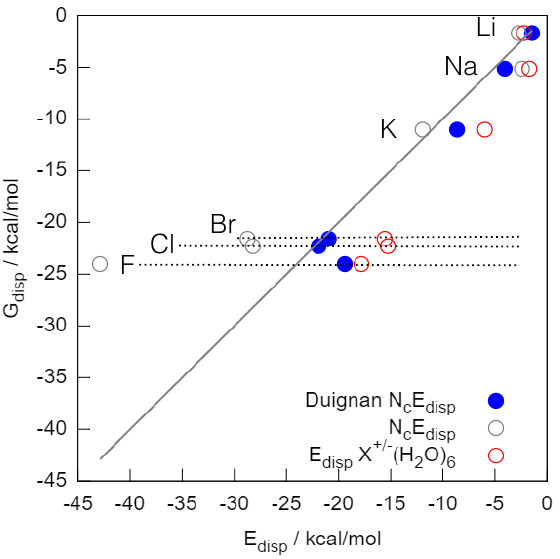
\includegraphics[width=0.8\linewidth]{images/ct_main/duignan_disp.png}
 \end{center}
 \caption[Ion/water dispersion energies and non-linear scaling]{\label{fig:duignan_disp}Figure adapted from Duignan et al.\cite{duignan2014collins}. 
 Figure highlights the non-linear scaling of interaction energy components, both N$_{c}$E$_{disp}$ estimates are too large to fit the continuum
 model described in the same reference. The SAPT2+3(CCD) results for explicitly modeled larger clusters I present here underestimate the dispersion 
 energy relative to the higher order estimate of G$_{disp}$ and so is the more physically consistent result. This demonstrates that interaction 
 energy components are not additive even within the first solvation shell. N$_{c}$ are experimental coordination numbers and E$_{disp}$ are dispersion
 energies from DFT-SAPT or SAPT2+3(CCD) depending on source.}
\end{figure}

  A term often left out of discussions of the SAPT interaction energy is the exchange component which is evaluated with an approximation
  in Psi4 that scales with the square of the overlap integral between basis functions centered on the separate monomers. This property allows for a quantitative 
  assessment of the degree of charge overlap within the clusters and is seen to track the charge transfer values from AIM in Table \ref{tab:ct_all} reasonably 
  well. A charge transfer component of the SAPT induction energy can be separated from polarization using one of the two methods discussed in Ref. \cite{stone2009ct} 
  and Ref. \cite{jeziorski2004regsapt,misquitta2013regsapt}. I discuss more on this later as well.

  The energetic analysis is complemented here with QTAIM descriptors highlighted in Table \ref{tab:dimer_aim}. As with the SAPT energies, each of the properties
  correlates with the strongly ionic/electrostatic nature of ion/water association (positive $\nabla\sur{2}\rho$ at the bond critical point (\emph{bcp}) and a 
  ratio of the magnitude of the largest attractive curvature to the repulsive curvature, $\frac{\left|\lambda\sous{1}\right|}{\lambda\sous{3}}$, less than unity). 
  However hydrogen-bonding within the AIM theory is characterized by an electrostatic presentation of the electron density curvature but a negative total energy
  density which is dominated by the potential energy density. This differs from a covalent linkage which  would also have a negative second derivative at the 
  \emph{bcp}. The large amount of electron density ($\rho$) located at the F\sur{-}(H\sous{2}O) dimer \emph{bcp} coupled with the negative total energy per charge
  is consistent with the uncharacteristically high induction and exchange contributions to the SAPT interaction energies relative to Cl\sur{-} and Br\sur{-}. This
  may offer some insight into the origin of the argument for the apparent chemical character of the interaction discussed in Refs. 
  \cite{collins2007review,mccoy2006prywaterf}. 
  
  It is evident that the F\sur{-} ion is much more strongly associated with the water than are the other halides likely owing to its small size and relatively 
  large proton affinity\cite{kim2002bigall}. This is also seen through the extent of charge penetration of the ion into the water ``electron cloud.'' I found 0.79 
  Bohr separation of the ion from the \emph{bcp} as compared to 1.32 and 1.43 Bohr for Cl\sur{-} and Br\sur{-}, respectively. However, an AIM analysis of a series 
  of halogen and hydrogen bonded complexes together with the reduced variational space (RVS) energy decomposition analysis (at the SCF level) revealed that the 
  decrease in the total energy density and increasing electron density at the intermolecular \emph{bcp} are principally due to a marked increase in attractive
  electrostatic interactions\cite{angelina2013cov}. In the RVS theory, charge transfer is considered a component of the chemical or covalent energy terms.

\begin{table}
 \begin{center}
 \begin{tabular}{cccccrc}
  \multicolumn{1}{c}{Ion} & \multicolumn{1}{c}{r(H\sous{2}O-\emph{bcp})} & \multicolumn{1}{c}{$\rho$} & \multicolumn{1}{c}{$\nabla^2\rho$} & \multicolumn{1}{c}{$\left|\lambda_{1}\right|/\lambda_{3}$} & \multicolumn{1}{c}{$H$/$\rho$} & \multicolumn{1}{c}{$\left|V\right|$/G} \tabularnewline
 \hline
  Li$^+$ & 2.16 & 0.0367 & 0.2984 & 0.17 &  0.3229 & 0.81 \tabularnewline
  Na$^+$ & 2.31 & 0.0249 & 0.1865 & 0.14 &  0.3212 & 0.79 \tabularnewline
  K$^+$  & 2.40 & 0.0213 & 0.1137 & 0.15 &  0.2101 & 0.81 \tabularnewline
  F$^-$  & 0.79 & 0.0882 & 0.1351 & 0.38 & -0.4848 & 1.56 \tabularnewline
  Cl$^-$ & 1.32 & 0.0291 & 0.0589 & 0.28 & -0.1456 & 1.22 \tabularnewline
  Br$^-$ & 1.43 & 0.0238 & 0.0472 & 0.26 & -0.1042 & 1.17 \tabularnewline
 \hline
 \end{tabular}
 \end{center}
 \caption[Atoms in molecules properties at \emph{bond critical point}]{\label{tab:dimer_aim} AIMAll output of several chemical indicators computed 
 at the intermolecular bond critical point (\emph{bcp}). 
 r(H\sous{2}O-\emph{bcp}) is the distance from the participating atom in the water molecule to the intermolecular \emph{bcp} and is a 
 measure of ion penetration. $\rho$ is the value of the density and $\nabla\sur{2}\rho$ the Laplacian at the \emph{bcp}. In the fourth 
 column, we report the ratio of the largest negative curvature (attraction) to the curvature along the bond path (repulsion). This is 
 typically interpreted as a measure of the local balance between potential and kinetic energies and is usually much less than unity for
 closed-shell, primarily electrostatic interactions. Additionally, we report the total energy density per unit charge and the ratio of 
 the potential to kinetic energy at the critical point. Hydrogen bonds in the AIM theory display largely electrostatic character in the
 Laplacian but somewhat chemical character in the energy terms. It is the uncharacteristically high amount of charge and enormously 
 negative total energy density which may fuel speculation that F\sur{-}/water interactions possess some chemical character. All  values 
 are reported in atomic units.}
\end{table}

  My discussion on charge transfer (or delocalization) in ion/water dimers focuses on the data presented in Table \ref{tab:dimer_ct}. 
  The sign convention used here is that charge depletion is given a negative value and accumulation a positive one. The data indicated that there was a loss 
  of charge for anions and an accumulation in the virtual orbitals of each of the cations. In the anion/water dimer, charge is also lost by the ion-bound hydrogen 
  (H\sous{b}) and populates a \emph{p}-state centered on the oxygen and also a diffuse Rydberg state bridging the oxygen and trailing hydrogen (resembling
  $\frac{1}{2}$ the lowest unoccupied molecular orbital, LUMO). 

\begin{table}
 \begin{center}
 \begin{tabular}{lrlrlrlrlrlr}
  A & $\delta$q(A) & A & $\delta$q(A) & A & $\delta$q(A) & A & $\delta$q(A) & A & $\delta$q(A) & A & $\delta$q(A) \tabularnewline
 \hline
  Li\sur{+} &  32.4 & O         &  117.0 & Na\sur{+} &  27.4 & O         &  86.2 & K\sur{+}  &  21.9 & O         &  68.3 \tabularnewline
            &       & H\sous{1} &  -74.7 &           &       & H\sous{1} & -56.8 &           &       & H\sous{1} & -45.1 \tabularnewline
            &       & H\sous{2} &  -74.7 &           &       & H\sous{2} & -56.8 &           &       & H\sous{2} & -45.1 \tabularnewline
  F\sur{-}  & -83.4 & O         &  191.3 & Cl\sur{-} & -62.1 & O         & 110.0 & Br\sur{-} & -62.5 & O         &  98.5 \tabularnewline
            &       & H\sous{b} & -174.3 &           &       & H\sous{b} & -77.3 &           &       & H\sous{b} & -60.7 \tabularnewline
            &       & H\sous{f} &   66.3 &           &       & H\sous{f} &  29.3 &           &       & H\sous{f} &  24.7 \tabularnewline
 \hline
 \end{tabular}
 \end{center}
 \caption[Atoms in molecules atomic charges for ion/water dimers]{\label{tab:dimer_ct} AIM-derived charge transfer values (in m\emph{e}, millielectrons) 
 for dimers computed with AIMAll. Negative values reflect charge loss, positive values reflect charge accumulation.}
\end{table}
  
  \noindent These features are illustrated in the electron density difference maps of Figures \ref{fig:f-6-r4aa-delrho}
  and \ref{fig:f-2-contour}. The oxygen amasses charge also in the cation/water dimers, drawing equal quantities of charge from the dangling hydrogens. About one 
  half of the charge exchanged in the weakest anion/water dimers (Cl\sur{-} and Br\sur{-}) is exchanged by even the most strongly bound cation/water dimer 
  (Li\sur{+}). These results compare well to the values obtained by Soniat et al. for Na\sur{+}, K\sur{+}, and Cl\sur{-}\cite{soniat2012ct}and we agree 
  qualitatively with trends which conclude charge transfer increases in the order of Br\sur{-} $<$ Cl\sur{-} $<$ F\sur{-} originating from studies
  of CT in halide/water dimers with L\"{o}wdin and natural bond orbital (NBO) charges\cite{kim1999bigf,kim2000smallall,kim2002bigall,hynes2000cthalides}. 

\begin{figure}
 \begin{center}
  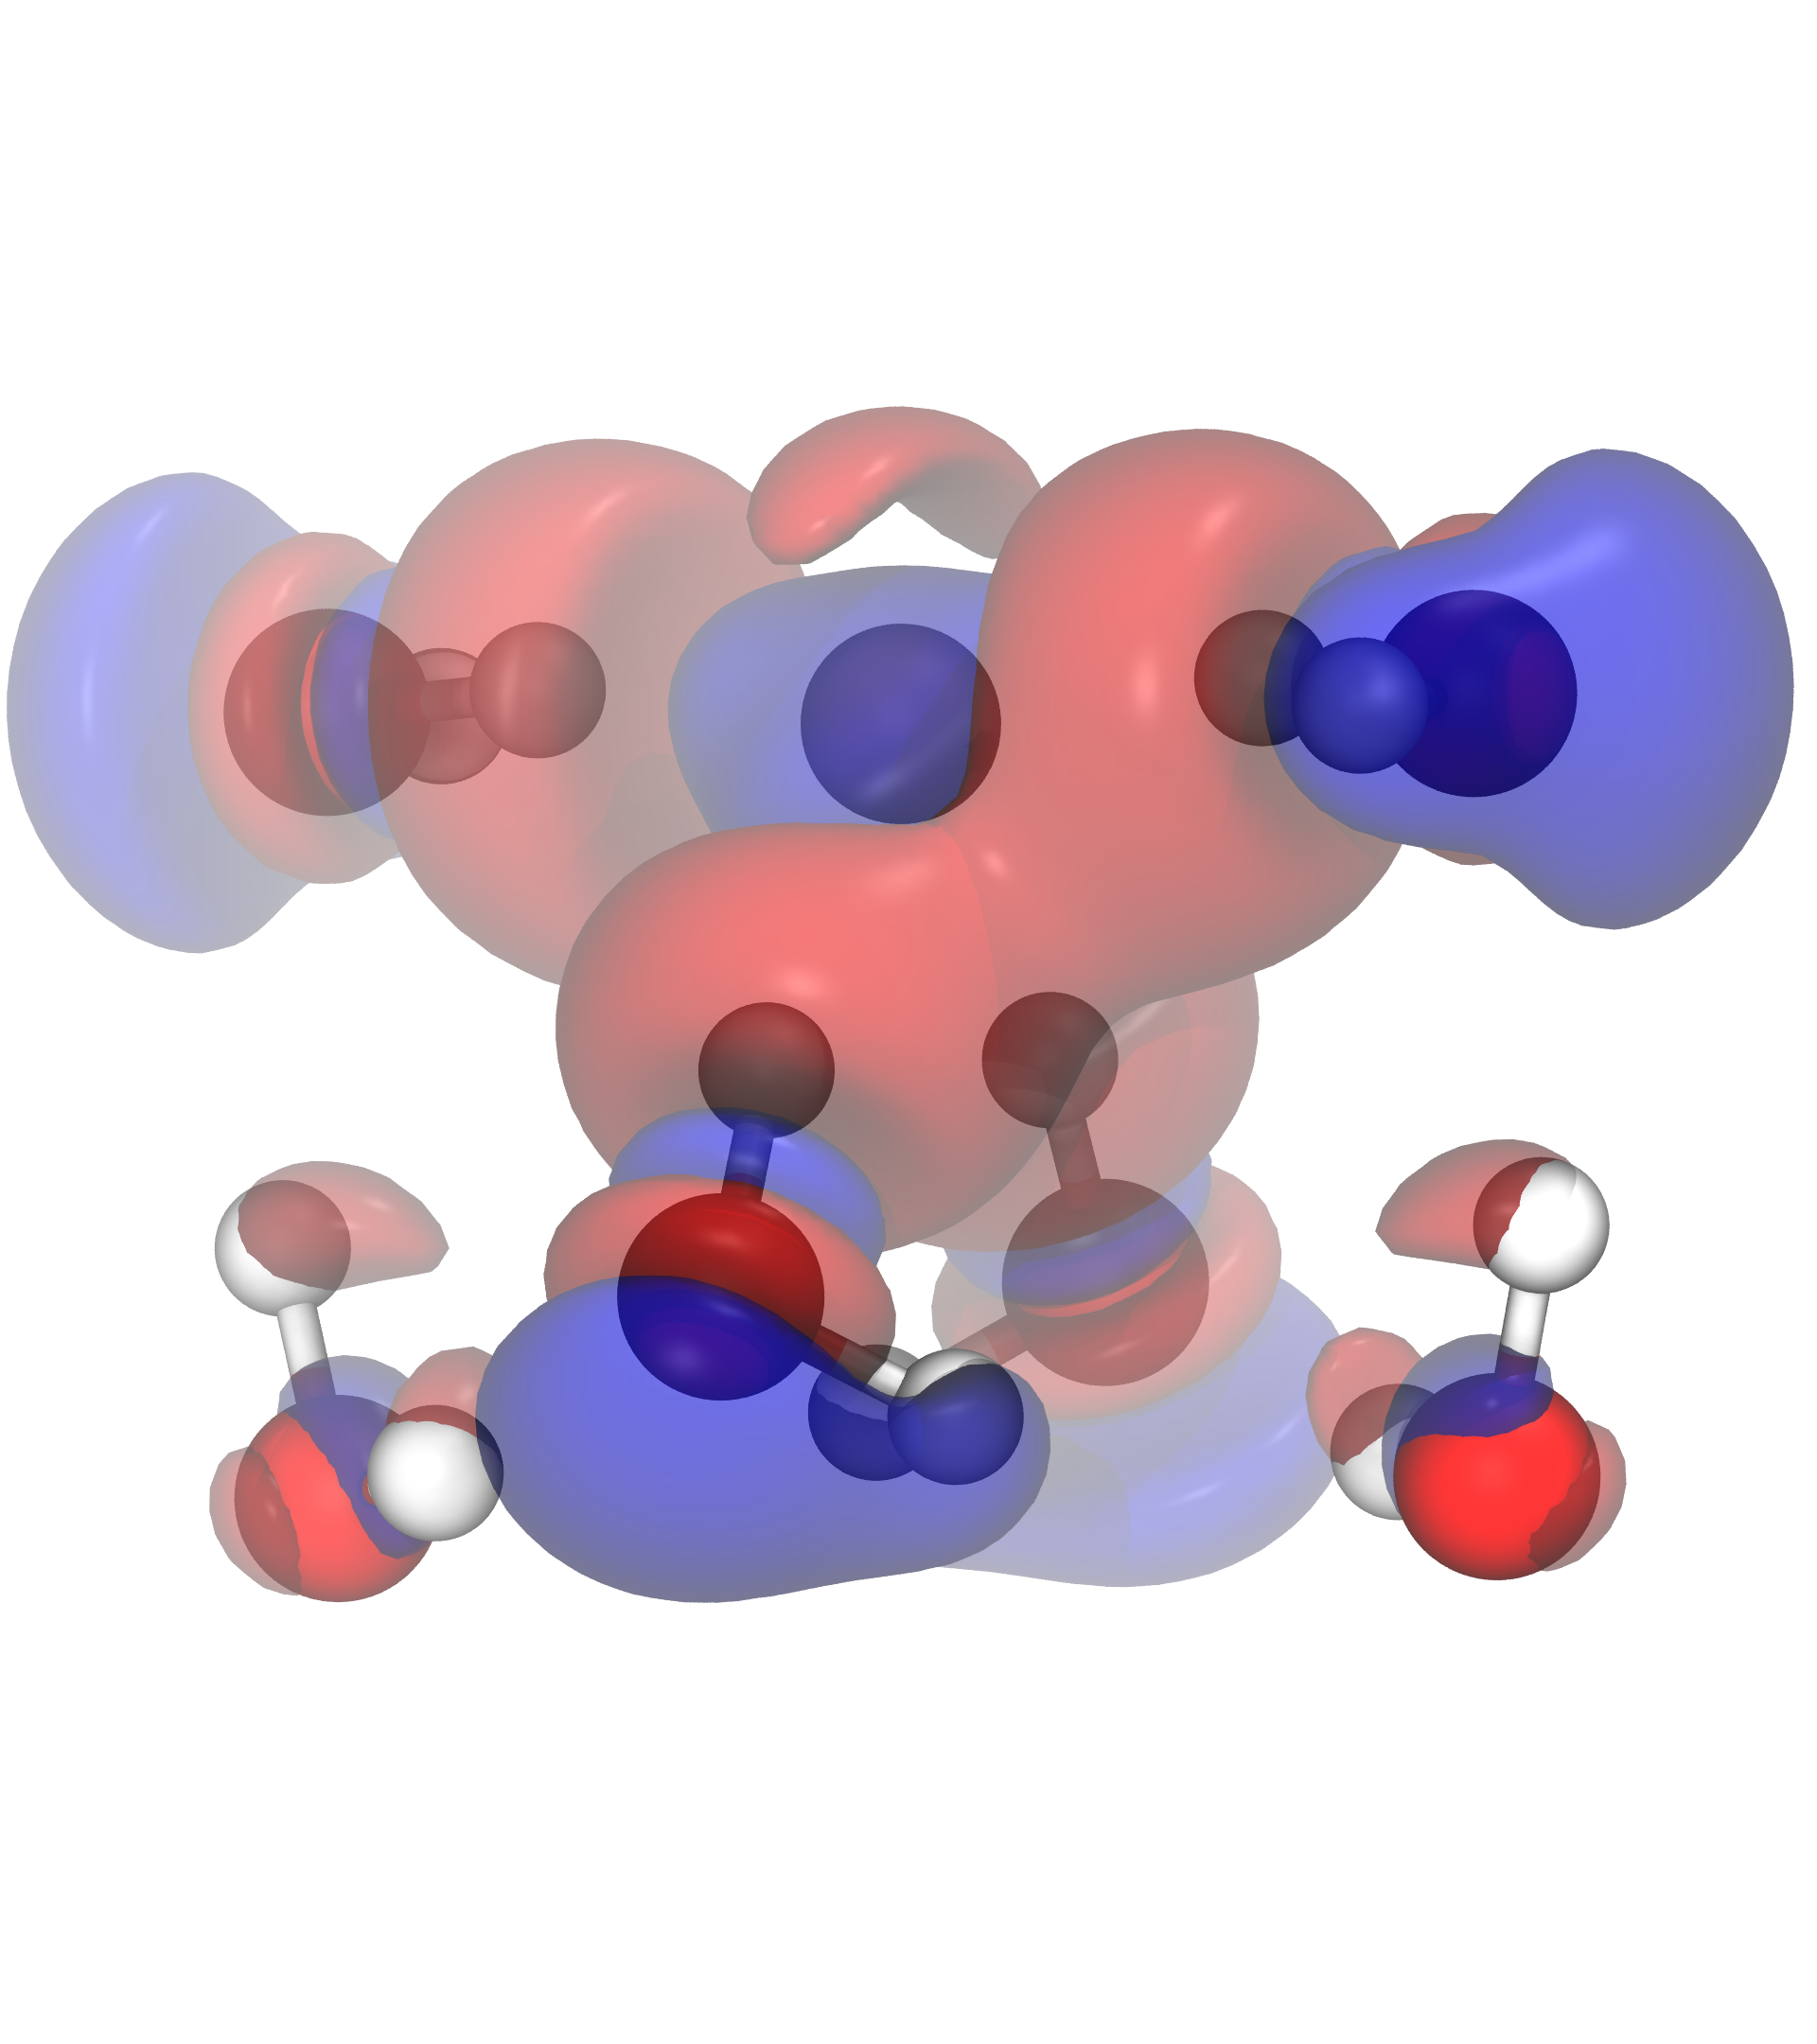
\includegraphics[width=0.98\linewidth]{images/ct_main/f-6-r4aa.png}
 \end{center}
 \caption[Electron density difference map in F$^{-}$(H$_{2}$O)$_{6}$]{\label{fig:f-6-r4aa-delrho}An electron density difference map of the $\pm$0.0022 \emph{e}
 isosurfaces of one of the F$^{-}$(H$_{2}$O)$_{6}$ clusters.}
\end{figure}

\begin{figure}
 \begin{center}
  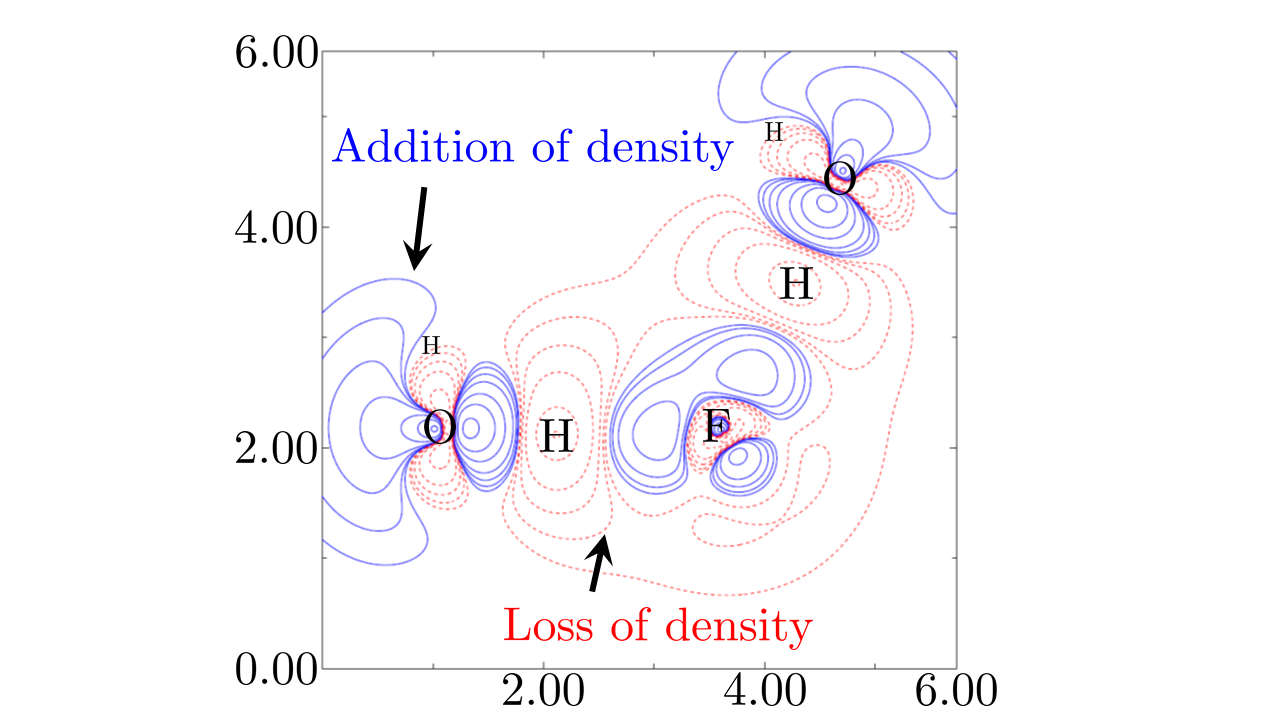
\includegraphics[width=0.98\linewidth]{images/ct_main/f-2-deltarho-Hb1XHb2.jpg}
 \end{center}
 \caption[Electron density difference contours in F$^{-}$(H$_{2}$O)$_{2}$]{\label{fig:f-2-contour}An electron density difference contour map of 
 F$^{-}$(H$_{2}$O)$_{2}$ clusters showing regions of charge accumulation and depletion.}
\end{figure}

  Moving beyond dimers into clusters, I'll be referring to Table \ref{tab:ct_all}. For trimers, there is a notable increase
  in the amount of charge redistribution throughout the system which falls well short of a doubling of the result for the dimers. Competition between ion/water
  versus water/water is not seen until reaching a coordination number of \emph{n} $=$ 3. We also point out that the trend observed for the anion/water dimers, 
  namely that charge transferred increases in the order Br\sur{-} $<$ Cl\sur{-} $<$ F\sur{-}, is in danger of reversing as the effect for F\sur{-} appears to 
  saturate rather quickly. This transition in anions is consistent with a study by Patel et al. in which they've found that for F\sur{-}/water clusters up to 
  \emph{n} $=$ 3, the ion polarizability was somewhat enhanced relative to the gas phase F\sur{-} polarizability\cite{patel2010polarizability}. Beyond a cluster 
  size of \emph{n} $=$ 3, the ion polarizability was reduced relative to the gas phase and as a consequence the observed ion-to-solvent transfer is quickly exhausted. 
  Figure \ref{fig:f-6-r4aa-delrho} shows that the water distorts the electron density of the ion towards poles directed at neighboring hydrogens. These polarized 
  electron-rich clouds are simply more willing to relinquish their charge from softer ions like Cl\sur{-} and Br\sur{-} than harder ones like F\sur{-}; and we 
  note that all anions eventually see a decrease in polarizability in the condensed phase limit -- a conclusion also reached by Masia\cite{masia2009polarize,masia2013polar} 
  and other researchers, see page 4 of Ref. \cite{ren2003amoeba} and the related discussion for more references.

  In clusters with more than 3 waters we see very little in the way of change from cation/water systems, maintaining a steady 60 to 80 millielectron draw from
  surrounding waters with a general preference for arrangements producing a high symmetry and maximizing the number of direct ion/water contacts. The same trend
  we observed for dimers is preserved in the micro-solvated states with Li\sur{+} drawing more charge than Na\sur{+} and K\sur{+}. However, the anion trend has
  reversed with Br\sur{-} shedding up to about 170 millielectrons while F\sur{-} has lost around 150 millielectrons at most. These figures are similar to the 
  results from Zhao, Rogers, and Beck where they found Cl\sur{-} to lose about 200 millielectrons\cite{rogers2010ctpolar}. Their calculations included the dipole 
  and quadrupole field of waters beyond the first hydration shell suggesting there may be a small amount of additional charge displaced as we approach the bulk
  limit. Finally, we note that the amounts of charge exchanged between the ions and water, just as we saw for the energies, did not increase linearly with each
  additional water -- in fact, most of these figures barely doubled with the addition of 5 more waters!

\begin{table}
 \begin{center}
  \begin{tabular}{lrlrlr}
   Cluster & $\delta$q(X\sur{\pm}) & Cluster & $\delta$q(X\sur{\pm}) & Cluster & $\delta$q(X\sur{\pm})\tabularnewline
  \hline
   \tabularnewline
   \multicolumn{2}{c}{\textbf{X\sur{\pm}(H\sous{2}O)\sous{1-4}}} & \multicolumn{2}{c}{\textbf{X\sur{\pm}(H\sous{2}O)\sous{4-5}}} & \multicolumn{2}{c}{\textbf{X\sur{\pm}(H\sous{2}O)\sous{5-6}}}\tabularnewline
   \tabularnewline
Li\sur{+} C\sous{2v}      &  32.4& F\sur{-} C\sous{1}                   &-138.7& Br\sur{-} R4A1             &-163.1 \\
Na\sur{+} C\sous{2v}      &  27.4& F\sur{-} C\sursous{\prime\prime}{1}  &-139.7& Br\sur{-} R4A              &-159.4 \\
K\sur{+} C\sous{2v}       &  21.9& F\sur{-} C\sous{4}                   &-134.6& Br\sur{-} R43f             &-157.8 \\
F\sur{-} C\sous{1}        & -83.4& F\sur{-} 3+1(C\sous{s})              &-139.2& Br\sur{-} R3AA\sur{\prime} &-162.3 \\
Cl\sur{-} C\sous{1}       & -62.1& Cl\sur{-} C\sursous{\prime}{1}       &-144.6& Br\sur{-} R5               &-149.4 \\
Br\sur{-} C\sous{1}       & -62.5& Cl\sur{-} C\sursous{\prime\prime}{1} &-143.0& Br\sur{-} R4f3             &-156.1 \\
                          &      & Cl\sur{-} C\sous{4}                  &-135.3&                            &       \\
Li\sur{+} D\sous{2d}      &  58.9& Br\sur{-} C\sursous{\prime}{1}       &-150.9& Li\sur{+} D\sous{2d}       &  82.0 \\
Na\sur{+} D\sous{2d}      &  49.7& Br\sur{-} C\sursous{\prime\prime}{1} &-149.1& Li\sur{+} 4+2(C\sous{s})   &  82.5 \\
K\sur{+} D\sous{2d}       &  37.6& Br\sur{-} C\sous{4}                  &-139.4& Li\sur{+} C\sous{2}        &  82.2 \\
F\sur{-} C\sous{2}        &-117.4&                                      &      & Na\sur{+} D\sous{2d}       &  77.2 \\
Cl\sur{-} C\sous{1}       &-100.0& Li\sur{+} C\sous{2}                  &  74.7& Na\sur{+} 4+2(C\sous{s})   &  76.9 \\
Br\sur{-} C\sous{1}       &-101.5& Li\sur{+} 4+1(C\sous{2})             &  82.4& Na\sur{+} C\sous{2}        &  74.7 \\
                          &      & Na\sur{+} C\sous{2}                  &  77.1& K\sur{+} D\sous{2d}        &  63.9 \\
Li\sur{+} D\sous{3}       &  74.4& Na\sur{+} 4+1(C\sous{2})             &  76.9& K\sur{+} 4+2(C\sous{s})    &  64.3 \\
Li\sur{+} 2+1(C\sous{2v}) &  58.6& K\sur{+} 4+1(C\sous{2})              &  62.6& K\sur{+} C\sous{2}         &  61.5 \\
Na\sur{+} D\sous{3}       &  65.4& K\sur{+} C\sous{2}                   &  59.0& F\sur{-} L3L3              &-150.9 \\
Na\sur{+} 2+1(C\sous{2v}) &  50.3& K\sur{+} 4+1(C\sous{1})              &  57.2& F\sur{-} R3ADA             &-145.7 \\
K\sur{+} D\sous{3}        &  51.5& F\sur{-} R3L2                        &-140.5& F\sur{-} R4AA              &-142.1 \\
K\sur{+} 2+1(C\sous{2v})  &  42.3& F\sur{-} R4L                         &-140.9& F\sur{-} Bf\sur{\prime}    &-140.0 \\
F\sur{-} C\sous{3}        &-128.4& F\sur{-} L3DL                        &-141.3& F\sur{-} R3AAL             &-141.6 \\
F\sur{-} 2+1(C\sous{s})   &-124.0& F\sur{-} R4A                         &-138.1& F\sur{-} Bf                &-138.9 \\
Cl\sur{-} C\sous{3}       &-121.1& F\sur{-} R43f                        &-137.4& Cl\sur{-} R4AA             &-163.8 \\
Cl\sur{-} 2+1(C\sous{s})  &-119.5& F\sur{-} R4L\sur{\prime}             &-141.4& Cl\sur{-} Bf\sur{\prime}   &-159.3 \\
Br\sur{-} C\sous{3}       &-124.2& F\sur{-} R3AA                        &-140.0& Cl\sur{-} Bf               &-158.7 \\
Br\sur{-} 2+1(C\sous{s})  &-123.1& Cl\sur{-} R4A1                       &-155.5& Cl\sur{-} Bd               &-150.6 \\
                          &      & Cl\sur{-} R4A                        &-151.2& Cl\sur{-} Bd\sur{\prime}   &-151.3 \\
Li\sur{+} S\sous{4}       &  81.2& Cl\sur{-} R43f                       &-150.0& Br\sur{-} R4AA             &-174.2 \\
Li\sur{+} 3+1(C\sous{2})  &  75.8& Cl\sur{-} R3AA\sur{\prime}           &-154.5& Br\sur{-} Bf\sur{\prime}   &-168.8 \\
Na\sur{+} S\sous{4}       &  76.0& Cl\sur{-} R5                         &-144.0& Br\sur{-} Bf               &-168.2 \\
Na\sur{+} 3+1(C\sous{2})  &  66.6& Cl\sur{-} R3AA                       &-149.4& Br\sur{-} Bd               &-158.2 \\
K\sur{+} S\sous{4}        &  61.4& Cl\sur{-} R4f3                       &-149.6& Br\sur{-} Bd\sur{\prime}   &-159.3 \\
K\sur{+} 3+1(C\sous{2})   &  53.5&                                      &      &                            &       \\
  \hline 
  \end{tabular}
 \end{center}
 \caption[Atoms in molecules partial charges on ions in all clusters]{\label{tab:ct_all} Charge transfer to ($\delta$q $>$ 0) or from 
 ($\delta$q $<$ 0) the ion measured in millielectrons for each complex examined. Note the increases are not linear when additional 
 waters are considered and the $\delta$q to cations and from F\sur{-} has already nearly plateaued when considering just the first 
 hydration shell.}
\end{table}

  An alternative approach to quantifying the amount of charge transfer was described by Belpassi and coworkers\cite{belpassi2009cd1,belpassi2010cd2} and is 
  particularly suited to examining charge displacement in or between linear or planar molecules. By slicing a cube file of the electron density difference 
  upon complexation into many planes perpendicular to the bond between the ion and nearest water atom and then integrating, I can examine the amount of charge
  transferred from one side of the plane to the other (direction depends on direction of integration, -z to +z or +z to -z). Belpassi has argued that between two
  interacting molecules there will be a minimum or a maximum in the curve which is the estimate of total charge transferred. Figure \ref{fig:belpassi} shows the
  charge displacement curve for all the ion/water dimers. The integration proceeds from -x to +x and so a positive value like we obtain for cations indicates 
  charge flow from the left side to the right (ion to water) and vice versa for negative values like that obtained for anions. The hills and valleys in this 
  curve coincide with the pattern of density accumulation or depletion like what is seen in Figure \ref{fig:f-2-contour} and provide an insightful new 
  perspective. Charge transfer values from this plot are as follows: 10.1 (Li\sur{+}), 10.1 (Na\sur{+}), 27.3 (K\sur{+}), 72.6 (F\sur{-}), 49.3 (Cl\sur{-}), 
  and 46.9 (Br\sur{-}) millielectrons which reverses the cation trend from that observed with AIM-derived partial charges but preserves the trend for anions.
  
\begin{figure}
 \begin{center}
  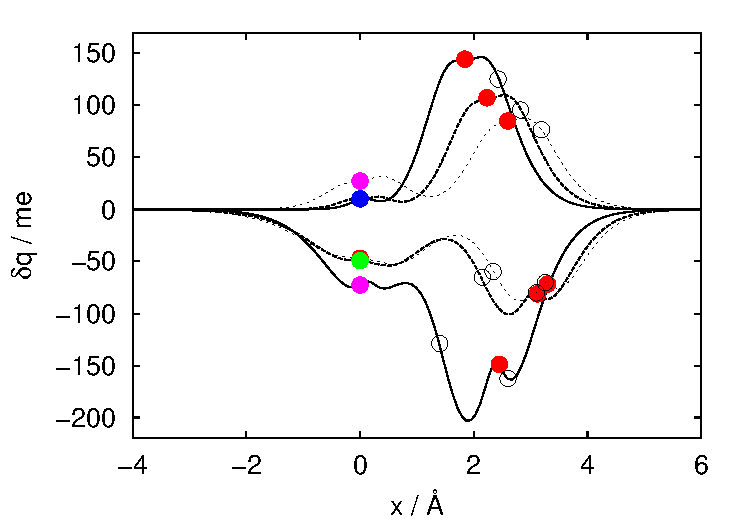
\includegraphics[width=0.98\linewidth]{images/ct_main/belpassi.pdf}
 \end{center}
 \caption[Charge displacement curves for ion/water dimers]{\label{fig:belpassi}Charge displacement curves following Refs. \cite{belpassi2009cd1,belpassi2010cd2}. 
  The curve indicates both direction and magnitude of charge passing through a moving plane perpendicular to the ion-water bond and so offers a unique
  perspective of charge redistribution in the dimers. Refs. \cite{belpassi2009cd1,belpassi2010cd2} and citations therein argue that an unambiguous 
  estimation of the charge transferred can be evaluated at the minimum/maximum appearing in the curve between the ion and the nearest water atom positions.
  The integration proceeds from left to right and so a positive value like we obtain for cations indicates charge flows from the right side to the 
  left (water to ion) and vice versa for negative values like those obtained for anions. All ions are located at x=0. Red and white circles not at
  the x=0 coordinate signify oxygen and hydrogen positions, respectively. Ions are colored magenta (F\sur{-}), green (Cl\sur{-}), red (Br\sur{-}), 
  larger red (Li\sur{+}), blue (Na\sur{+}), and magenta (K\sur{+}).}
\end{figure}
  
  \subsection{\label{ch3:sec2:level1:chasm2}Energy stabilization due to charge transfer}
  Tables \ref{tab:small_clust} and \ref{tab:3_clust} highlight the significant enhancement in basis set independence that regularization affords.
  Charge transfer energies are reported for basis sets ranging from a double-$\zeta$ through to a quadruple-$\zeta$ quality, yet exhibit little
  variance. This consistency is maintained as additional waters are added to create high or even low symmetry arrangements (see also Tables 
  \ref{tab:small_clusters}--\ref{tab:6_clusters}, with (X\sur{\pm}(H\sous{2}O)\sous{n}; \emph{n} = 1, \dots, 6)). However, there's an issue with
  these figures that was also observed by Lao et al.\cite{lao2016cdftsapt}. The cation/water dimers are considered to be a trivial case, with 
  the strength of polarization and charge transfer interactions increasing in the order of K\sur{+} < Na\sur{+} < Li\sur{+}, complimenting the
  decrease in ion/water distance. However, CT\sursous{(2)}{SM09}, CT\sursous{(2)}{Reg, aDZ}, and CT\sursous{(2)}{Reg, pc1} displayed a tendency
  to go positive for small cation/water clusters and only slightly negative for the largest clusters. This is with the exception of Na\sur{+} which
  always produced a positive charge transfer energy, regardless of cluster size, method, or basis set used. Ordering of the cation energies using
  the SM09 method trend varied with cluster size but remained constant among regularized energies as K\sur{+} > Na\sur{+} > Li\sur{+} (where K\sur{+} 
  is merely the least \emph{unfavorable}). It's also interesting to note that while Li\sur{+}/water and K\sur{+}/water energies became more negative 
  with increasing cluster size, the regularized energies increased.
  
\begin{table}
 \begin{center}
  \begin{tabular}{lcccccc}
   \hline
   \hline
    Cluster & CT\sursous{(2)}{Reg, aDZ} & CT\sursous{(2)}{Reg, pc1} & CT\sursous{(2)}{Reg, aTZ} & CT\sursous{(2)}{Reg, pc2} & CT\sursous{(2)}{Reg, dTZ} & CT\sursous{(2)}{Reg, dQZ} \tabularnewline
   \hline
    \tabularnewline
    \multicolumn{7}{c}{\textbf{X\sur{\pm}(H\sous{2}O)}}  \tabularnewline
    \tabularnewline
    Li\sur{+} C\sous{2v} & 1.38 & 1.28 & 1.58 & 1.53 & 1.59 & 1.58 \tabularnewline
    Na\sur{+} C\sous{2v} & 0.45 & 0.33 & 0.51 & 0.49 & 0.46 & 0.50 \tabularnewline
    K\sur{+}  C\sous{2v} & 0.06 & 0.04 & 0.06 & 0.05 & 0.06 & 0.06 \tabularnewline
    F\sur{-}  C\sous{1}  &-4.15 &-4.20 &-4.10 &-4.24 &-4.14 &-4.09 \tabularnewline
    Cl\sur{-} C\sous{1}  &-0.67 &-0.70 &-0.62 &-0.62 &-0.62 &-0.60 \tabularnewline
    Br\sur{-} C\sous{1}  &-0.50 &-0.52 &      &-0.46 &-0.45 &-0.44 \tabularnewline

    \tabularnewline
    \multicolumn{7}{c}{\textbf{X\sur{\pm}(H\sous{2}O)\sous{2}}}  \tabularnewline
    \tabularnewline
    Li\sur{+} D\sous{2d} & 2.11 & 2.11 & 2.35 & 2.31 & 2.36 & 2.34 \tabularnewline
    Na\sur{+} D\sous{2d} & 0.83 & 0.65 & 0.91 & 0.88 & 0.86 & 0.90 \tabularnewline
    K\sur{+}  D\sous{2d} & 0.18 & 0.14 & 0.18 & 0.17 & 0.17 & 0.17 \tabularnewline
    F\sur{-}  C\sous{2}  &-4.70 &-4.77 &-4.59 &-4.77 &-4.63 &-4.57 \tabularnewline
    Cl\sur{-} C\sous{1}  &-1.10 &-1.15 &-1.01 &-1.02 &-1.01 &-1.00 \tabularnewline
    Br\sur{-} C\sous{1}  &-0.84 &-0.88 &      &-0.77 &-0.76 &-0.75 \tabularnewline
   \hline
   \hline
  \end{tabular}
 \end{center}
 \caption[Charge transfer energies for ion/water clusters with \emph{n} = 1 and 2]{\label{tab:small_clust} Charge transfer energies from regularized 
 SAPT computed (by column) with the (aug-)cc-pVDZ, (aug-)pc-1, (aug-)cc-pVTZ, (aug-)pc-2, 
 def2-TZVPP(D), and def2-QZVPP(D) basis sets. All values expressed in kcal/mol. Some entries are left blank due to limitations with the software.}
\end{table}

\begin{table}
 \begin{center}
  \begin{tabular}{lcccccc}
   \hline
   \hline
    Cluster & CT\sursous{(2)}{Reg, aDZ} & CT\sursous{(2)}{Reg, pc1} & CT\sursous{(2)}{Reg, aTZ} & CT\sursous{(2)}{Reg, pc2} & CT\sursous{(2)}{Reg, dTZ} & CT\sursous{(2)}{Reg, dQZ} \tabularnewline
   \hline
    \tabularnewline
    \multicolumn{7}{c}{\textbf{X\sur{\pm}(H\sous{2}O)\sous{3}}}  \tabularnewline
    \tabularnewline
    Li\sur{+} 2+1(C\sous{2}) & 2.20 &  2.13 & 2.41 & 2.36 & 2.43 & 2.41 \tabularnewline
    Li\sur{+} D\sous{3}      & 2.27 &  2.24 & 2.50 & 2.46 & 2.52 & 2.50 \tabularnewline 
    Na\sur{+} 2+1(C\sous{2}) & 0.85 &  0.69 & 0.93 & 0.90 & 0.88 & 0.92 \tabularnewline
    Na\sur{+} D\sous{3}      & 1.03 &  0.83 & 1.12 & 1.08 & 1.07 & 1.11 \tabularnewline
    K\sur{+}  2+1(C\sous{2}) & 0.10 &  0.08 & 0.11 & 0.10 & 0.10 & 0.10 \tabularnewline
    K\sur{+}  D\sous{3}      & 0.24 &  0.22 & 0.25 & 0.24 & 0.24 & 0.25 \tabularnewline
    F\sur{-}  2+1(C\sous{s}) &-5.34 & -5.41 &-5.24 &-5.42 &-5.29 &      \tabularnewline
    F\sur{-}  C\sous{3}      &-4.31 & -4.38 &-4.18 &-4.33 &-4.21 &      \tabularnewline 
    Cl\sur{-} 2+1(C\sous{s}) &-1.48 & -1.55 &-1.39 &-1.39 &-1.38 &      \tabularnewline
    Cl\sur{-} C\sous{3}      &-1.21 & -1.29 &-1.09 &-1.13 &-1.11 &      \tabularnewline
    Br\sur{-} 2+1(C\sous{s}) &-1.15 & -1.20 &      &-1.07 &-1.05 &      \tabularnewline
    Br\sur{-} C\sous{3}      &-0.94 & -1.00 &      &-0.87 &-0.85 &      \tabularnewline
   \hline 
   \hline
  \end{tabular}
 \end{center}
 \caption[Charge transfer energies for ion/water clusters with \emph{n} = 3]{\label{tab:3_clust} Charge transfer energies from regularized SAPT 
 computed (by column) with the (aug-)cc-pVDZ, (aug-)pc-1, (aug-)cc-pVTZ, (aug-)pc-2, 
 def2-TZVPP(D), and def2-QZVPP(D) basis sets. All values expressed in kcal/mol. Some entries are left blank due to limitations with the software.}
\end{table}  

  Tables \ref{tab:small_clusters}--\ref{tab:6_clusters} do however suggest that electron correlation offers a bit of improvement as it was 
  always evaluated to be negative, but surely does not improve the reliability of the results from either method. The infinite-order correction 
  to the induction energies is argued to account for charge transfer effects wrapped up in higher order effects not captured in the 2\sur{nd}-order
  expansion\cite{lande2015cdftct}. As with electron correlation, this drives the CT energies more negative with the exception of Na\sur{+}, for 
  which the $\delta$\sursous{(2)}{HF}(DCBS) term is curiously positive. The same was observed here as well\cite{lao2016cdftsapt}.

  Anions consistently produced more reasonable values and in the proper ordering (from \emph{least} to \emph{most} favorable): Br\sur{-} < 
  Cl\sur{-} < F\sur{-}. Similar to what I observed for the atoms-in-molecules charge populations for the anions, the energies stagnated beyond
  \emph{n} $>$ 3 for F\sur{-} -- however, without falling behind either Cl\sur{-} or Br\sur{-}. CT\sursous{(2)}{SM09} energies hovered around
  twice the energies predicted by the regularized method, especially for larger clusters. This is an interesting result as the saturation in 
  the amount of charge transfer observed particularly for F\sur{-} might have been expected to lead to better agreement between the SM09 and
  reg-SAPT methods.

  These results are also visualized in Figure \ref{fig:ct_energy}. Though here, we are able to decompose the CT energies even further into 
  donor $\rightarrow$ acceptor and donor $\leftarrow$ acceptor contributions (here, donor and acceptor refer to electrons, not 
  protons)\cite{jeziorski1994sapt}. The CT\sur{(2)}(X$\leftarrow$W) values settled near 0. kcal/mol for the entire range of cation/water clusters
  considered. This is to be expected however, as CT\sur{(2)}(X$\leftarrow$W) represents the charge transfer energy change from the water polarizing
  the ion. This leaves only the water-to-ion transfer which appeared to somewhat destabilize these complexes as discussed previously. For the
  anion/water clusters, inductive effects due to charge transfer appeared beneficial in both directions, though with the larger 
  portion originating from the ion $\leftarrow$ water term. As discussed previously, it is apparent that CT\sur{(2)}(X$\leftarrow$W) has saturated 
  for F\sur{-} already by \emph{n} $=$ 3, while both Cl\sur{-} and Br\sur{-} appeared to not yet converge.
  
\begin{figure}
 \begin{center}
  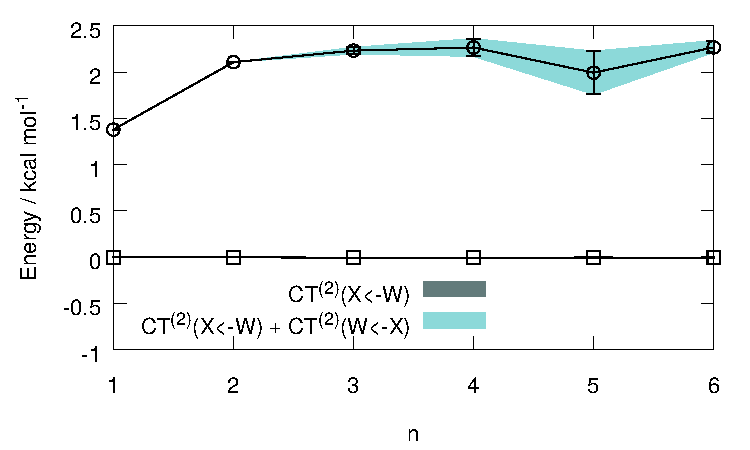
\includegraphics[width=0.48\linewidth]{images/ct_energy_data/e2ind_ct2_plots/pdf/li-ct.pdf}
  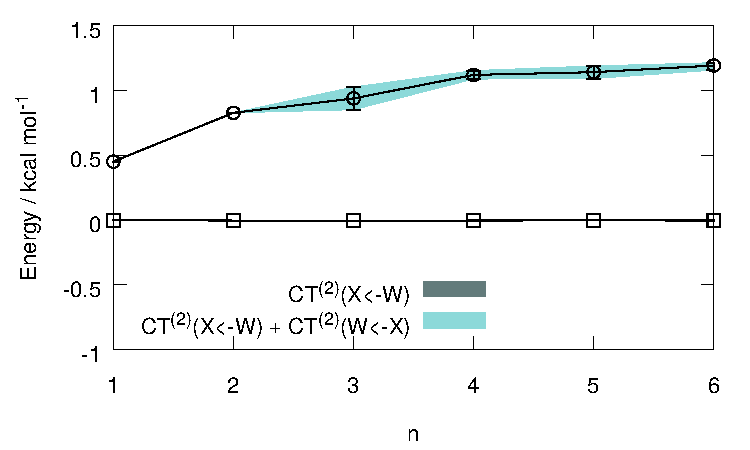
\includegraphics[width=0.48\linewidth]{images/ct_energy_data/e2ind_ct2_plots/pdf/na-ct.pdf} \\
  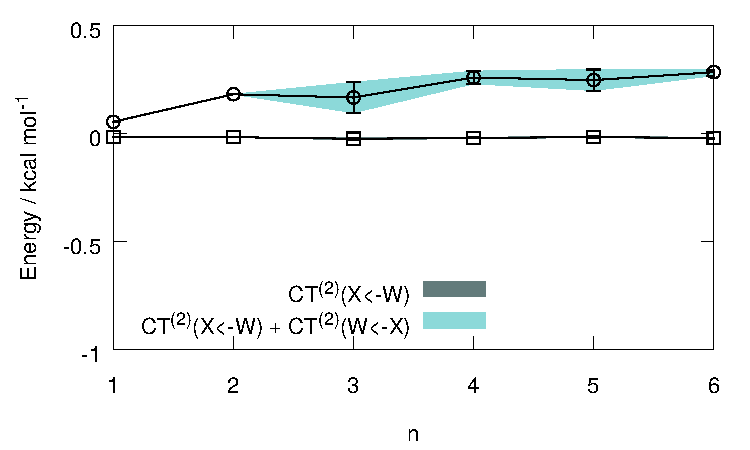
\includegraphics[width=0.48\linewidth]{images/ct_energy_data/e2ind_ct2_plots/pdf/k-ct.pdf} 
  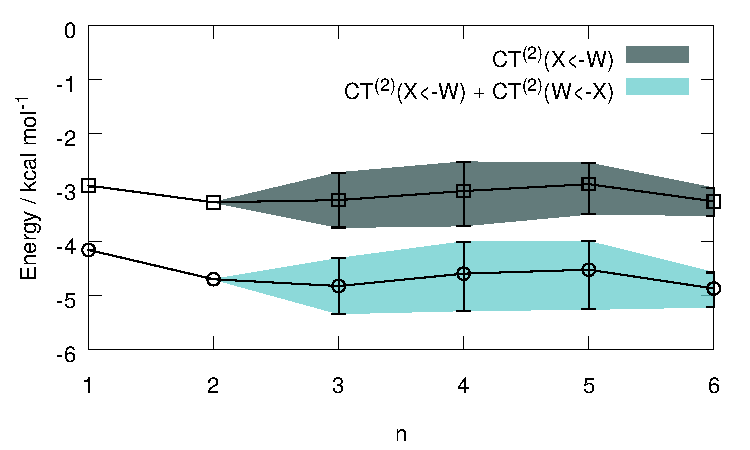
\includegraphics[width=0.48\linewidth]{images/ct_energy_data/e2ind_ct2_plots/pdf/f-ct.pdf} \\
  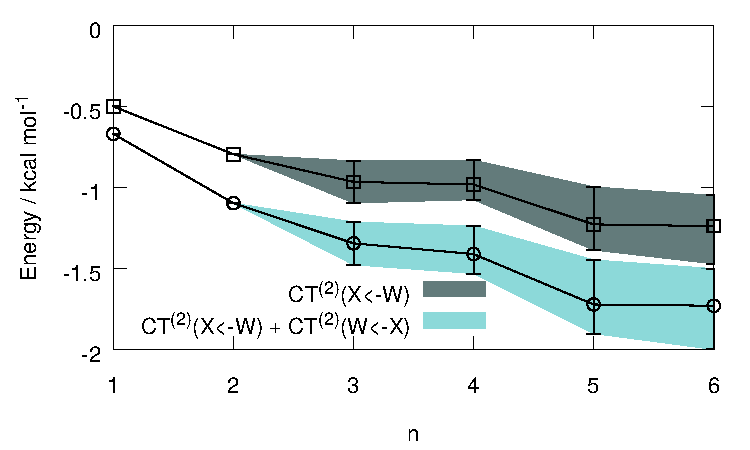
\includegraphics[width=0.48\linewidth]{images/ct_energy_data/e2ind_ct2_plots/pdf/cl-ct.pdf} 
  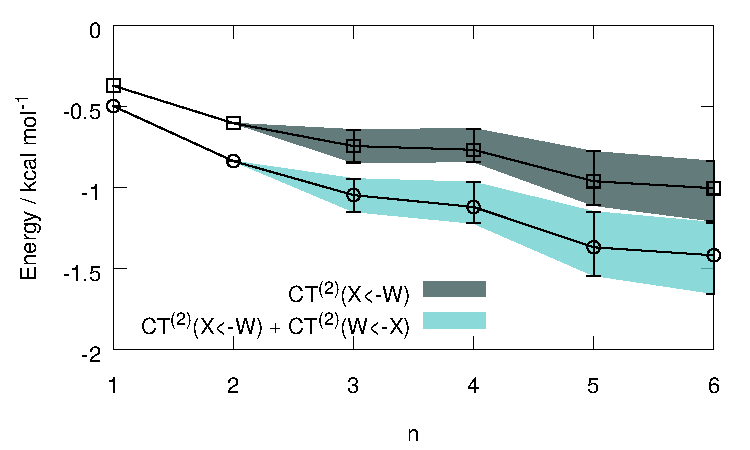
\includegraphics[width=0.48\linewidth]{images/ct_energy_data/e2ind_ct2_plots/pdf/br-ct.pdf} \\
 \end{center}
 \caption[Separate ion and solvent contributions to charge transfer energy]{\label{fig:ct_energy}Ionic and solvent contributions to total 
 charge transfer energies computed with the aug-cc-pVDZ basis set.
 CT\sur{(2)}(X$\leftarrow$W) is the charge transfer energy change for the ion induced by the permanent multipoles of the surrounding 
 solvent. Solvent effects due to the neighboring ion are taken as the difference in CT\sur{(2)}(X$\leftarrow$W) + CT\sur{(2)}(W$\leftarrow$X) 
 and the included ionic contribution. A solid line with points at each coordination number (\emph{n}) traces the mean values across all 
 structures and the shaded region is bounded by the maximum and minimum for a given cluster size. These extrema are identical to those found 
 in Tables 2-5. The procession of the ions from top left to bottom right is as follows: Li\sur{+}, Na\sur{+}, K\sur{+}, F\sur{-}, 
 Cl\sur{-}, and Br\sur{-}.}
\end{figure}

  So why the positive charge transfer energies? Table \ref{tab:liconverge} tells us that for the Li\sur{+}/water dimer, the presence of a regularizing
  potential even in the limit of large $\eta$ more aggressively screens the repulsive contributions than it does the attractive ones. This leads to the 
  systematic overestimation of the repulsive contribution, which may make this method more promising as an upper bound of the polarization energy instead 
  of an estimate of the charge transfer energy.
  
\begin{table}
 \begin{center}
 \resizebox{\columnwidth}{!}{
  \begin{tabular}{cccccccccc}
   \hline
   \hline
    $\eta$   & E\sursous{(2)}{tot,r} & E\sursous{(2)}{tot,r}(Reg) & CT\sur{(2)} & E\sursous{(2)}{ind,r} & E\sursous{(2)}{ind,r}(Reg) & CT\sursous{(2)}{attr} & E\sursous{(2)}{ex-ind,r} & E\sursous{(2)}{ex-ind,r}(Reg) & CT\sursous{(2)}{rep} \tabularnewline
   \hline
    2.0     &-11.43  &-12.54    &1.11  &-19.42  &-14.14   &-5.28    &7.99    &1.60   &6.39 \tabularnewline
    3.0     &-11.43  &-12.81    &1.38  &-19.42  &-15.47   &-3.95    &7.99    &2.66   &5.32 \tabularnewline
    4.0     &-11.43  &-12.82    &1.39  &-19.42  &-16.25   &-3.17    &7.99    &3.42   &4.56 \tabularnewline
    5.0     &-11.43  &-12.77    &1.34  &-19.42  &-16.76   &-2.66    &7.99    &3.99   &4.00 \tabularnewline
    6.0     &-11.43  &-12.70    &1.27  &-19.42  &-17.12   &-2.30    &7.99    &4.42   &3.56 \tabularnewline
    8.0     &-11.43  &-12.56    &1.12  &-19.42  &-17.61   &-1.82    &7.99    &5.05   &2.94 \tabularnewline
    10.0    &-11.43  &-12.44    &1.00  &-19.42  &-17.92   &-1.51    &7.99    &5.48   &2.51 \tabularnewline
    20.0    &-11.43  &-12.08    &0.64  &-19.42  &-18.59   &-0.83    &7.99    &6.51   &1.47 \tabularnewline
    100.0   &-11.43  &-11.60    &0.17  &-19.42  &-19.23   &-0.19    &7.99    &7.62   &0.37 \tabularnewline
    1000.0  &-11.43  &-11.45    &0.02  &-19.42  &-19.40   &-0.03    &7.99    &7.94   &0.04 \tabularnewline
   \hline 
   \hline
  \end{tabular}
  }
 \end{center}
 \caption[Regularized SAPT energy with varying screening width]{\label{tab:liconverge} Illustration of the effect of regularization in SAPT 
 induction energy components for Li\sur{+}(H\sous{2}O) 
 (units of kcal mol\sur{-1}). The exchange part of the interaction is more significantly impacted by the screening potential than is the 
 attractive part -- since CT\sur{(2)} is described nearly exclusively by the polarization of the water molecule, it is seen that the 
 positive CT energy results from the omission of the stresses leading to water-to-ion charge delocalization. Here E\sursous{(2)}{tot,r} is 
 the total induction energy, which is divided in other columns to the attractive induction term and the repulsive exchange coupled term. 
 E\sursous{(2)}{tot,r}(Reg) and CT\sur{(2)} are similarly decomposed. The full CT energy and its components are merely the differences 
 from the two columns preceding it. The table itself was slightly rescaled to fit the dimensions of the page.}
\end{table}

  There is much interest in correlating charge transfer energies in anion/water clusters with the degree of solvation asymmetry in the first 
  hydration shell. While it is known that the softer anions (e.g., Cl\sur{-}, Br\sur{-}, and I\sur{-}) tend to prefer a highly asymmetric 
  first solvation shell, the reduction in polarizability observed in the transition from gas phase to condensed phase for each
  ion\cite{masia2013polar,patel2010polarizability} (presumably from charge transfer to solvent making the ion appear `harder') has been seen to
  decrease solvation anisotropy when modeled with static multipoles using the AMOEBA polarizable force field\cite{rogers2010ctpolar} and the
  polarizable and fluctuating charge model of Soniat et al.\cite{soniat2012ct}. It would be quite useful to observe that semi-/internal bound
  clusters are selected for with enhanced CT energies relative to the surface-bound configurations, see the discussion on this in Ref.
  \cite{kim2002bigall}. Assuming the anion figures to be at least qualitatively accurate, the internal-bound configurations for 
  F\sur{-}(H\sous{2}O)\sous{6} (L3L3, R3AAL, and R3ADA) were selected over the surface bound states by both energy partitioning schemes.
  Perhaps the constrained density functional theory approach of Lande et al.\cite{lande2015cdftct} which showed greater consistency with
  cation/water dimers\cite{lao2016cdftsapt} than the SM09 method or the absolutely localized molecular orbital approach of Khaliullin et 
  al.\cite{khaliullin2008almo} can provide more solid answers using even larger clusters since it is based on DFT.

  This is all not to say that regularized SAPT isn't useful, rather it may be more fitting to interpret these energies in a similar manner to
  the polarized orthogonal local molecular orbitals (polMO) approach of Azar et al.\cite{azar2013polmo}. Where the polMO method has been shown
  to underestimate polarization effects, giving a lower bound to the polarization energy, reg-SAPT may reasonably be taken as an upper bound 
  for the polarization energy and lower bound for the charge transfer energy. My discussion on Table \ref{tab:liconverge} clearly demonstrated 
  that the reg-SAPT method overestimated the relaxation in the induction-exchange coupled term even in the limit of a vanishing conditioning
  potential. This effect leads to the positive CT energies observed in both the SM09 and reg-SAPT methods. It vanished with the CT energy itself
  in the SM09 method, but was retained in the reg-SAPT method which greatly improved the stability of the result with increasing basis set size.

  \section{\label{ch3:sec3:level1}Conclusions}
  My efforts show that there is an appreciable degree of ion specificity in the interactions between ions and associated solvent molecules. 
  These interactions are principally electrostatic in character. This is not to discount the role of induction (which is part polarization and
  part charge transfer) and dispersion which have been found by Rogers et al.\cite{rogers2010ctpolar,rogers2010qct}, Masia\cite{masia2013polar}, 
  Duignan et al.\cite{ninham2011review,duignan2013continuum1,duignan2013continuum2,duignan2014ion,duignan2014collins}, and 
  others\cite{collins2007review,soniat2012ct,soniat2014ct_surf,yao2014ct_diffusion,soniat2015znmg,soniat2015proton} to be of importance as well. The
  current study suggests up to $\approx\frac{1}{3}$ of the attractive contributions to the SAPT interaction energy arise from these 
  non-electrostatic forces. Despite the high level of complexity that has been found to be involved in ionic interactions, recent studies have 
  concluded that the effect of monovalent ions on water is surprisingly localized\cite{beck2011local,williams2012nanodrops}. I find evidence as
  well, with dispersion, charge transfer, and polarization showing signs of (near) saturation just within the first solvation shell. This invites 
  the possibility that more distant interactions can be treated with a coarse-grained or even continuum solvation model. Di- and trivalent ions 
  present yet another significant obstacle as the ion effects on the hydrogen bonding network in water have been found to be more
  far-reaching\cite{williams2012nanodrops,williams2015trivalent,williams2015crystal}.
  
  I have also conducted an in-depth analysis of small ion/water clusters in an effort to better understand what role(s) partial charge transfer between
  the ion and waters is expected to play. In particular, I was motivated by the recent attempts to develop fluctuating charge models which incorporate
  solute/solvent charge transfer and the suspected role this interaction may play in reshaping/restructuring the solvation shell around ions. This work
  explored the use of two approximate methods developed within the symmetry adapted perturbation theory to disentangle the charge transfer and 
  polarization energies from the total induction energy. I found the SM09 method based on differences in the induction term computed in the dimer- 
  and monomer-centered basis sets tended to overestimate the charge transfer energy relative to a method employing the use of regularized nuclear
  potentials to filter out charge transfer (which takes the place of the monomer-centered calculation). Charge transfer energies in anion/water clusters
  were found to be negative as expected, while cation/water clusters gave either positive or negative but very small energies. I showed that this effect
  was due to the regularizing potential overestimating the relaxation of the exchange-induction term even in the limit of the full Coulomb operator. I
  hypothesized that the regularized SAPT method may be better suited to providing an upper bound for the polarization energy rather than an estimate of the 
  charge transfer energy. However, assuming the relative values for a given ion to be qualitatively accurate, I observed that both partitioning schemes
  predicted that F\sur{-} would prefer internal-bound states relative to surface binding in the \emph{n} $=$ 6 clusters. This behavior is consistent with
  the prediction of previous simulations which saw reduced solvation anisotropy when including charge transfer explicitly or mimicking it by reducing the
  ion polarizability. A more thorough study would be needed to correlate the two with greater certainty and we discuss alternative approaches which may,
  in time, help us address this question.

\end{sie}